\chapter{Kapitel I - NoSQL - Grundlegende technologische Aspekte}
\section{Programmierschnittstellen}

\subsection{Komplexe Datenstrukturen}
\subsubsection{XML}
XML ist eine Abkürzung für Extensible Markup Language, die im Jahr 1998 erfinden wurde. der Herr. Helmut Vonhoegen definiert der XML als erste frei verfügbares Format für strukturierte Daten, unabhängig von bestimmten Plattformen und Anwendungen. Auch als Format für den Datenaustausch etabliert. XML ist auch ein universelles Datenbeschreibungsformat, weil es als einer der Web-Standards gilt, die vom W3C standardisiert wurden, weil es eine bessere Strukturierung des Dokuments ermöglicht und es auch erlaubt, die Dokumente im Web zu tauchen, was seine Besonderheit ausmacht. Die XML ist wegen ihrer Einfachheit sehr nützlich, aber auch, weil sie unabhängig von jeder Plattform, Anwendung, Kodierung, Protokoll usw. ist. Um XML besser zu verstehen, ist es wichtig, einen Blick in seine Vergangenheit zu werfen.

\textit{\textbf{Historik}}

die Sprache XML ist von den beiden Sprachen SGML und HTML abgeleitet. SGML (Standard Generalized Markup Language), der Vorläufer von HTML und XML, war für die Strukturierung von Dokumenten mit Hilfe von Tags gedacht, hatte aber den großen Nachteil, dass es nicht für das Web erweiterbar war und somit die Sprache HTML, um alle Informationen im Web zugänglich zu machen.  HTML ist wie wir alle wissen, eine Sprache, die es erlaubt Seiten zu erstellen, die im Web angezeigt werden können. Aber der Nachteil von HTLM ist, dass es Fakten und Formen vermischt.Als gemeinsamen Punkt können wir festhalten, dass HTML und XML zwei Sprachen sind, die sich am Text orientieren und Tags bilden, die es erlauben, Daten strukturell zu organisieren. Daraus wird XML geboren. 

Die Idee hinter der Schaffung von XML war, etwas zu haben, das Inhalt von Formen trennt und auch über das Web zugänglich ist. Während die Tags in HTML in erster Linie festlegen, in welche Form Inhalte in einem entsprechenden Medium ausgegeben werden sollen, wird mit XML versucht, die Bedeutung von Daten so festzulegen, dass nicht nur Menschen, sondern auch Maschinen damit etwas anfangen können.\cite{helmut32}

\textit{\textbf{Anwendung}}

Um ein syntaktisch korrektes XML-Dokument zu schreiben, müssen zunächst zwei grundlegende Prinzipien beachtet werden. Erstens muss das XML-Dokument wohlgeformt sein (Well form). Das bedeutet, dass erstens die Regeln und Konventionen für das Schreiben der Tags eingehalten werden müssen, die vom W3C vorgegeben werden, und zweitens muss auch die Verschachtelungsreihenfolge der Tags beachtet werden. Das zweite Prinzip ist, dass das XML-Dokument gültig sein muss. Dies ist ein optionaler Schritt, der aber notwendig ist, wenn wir möchten, dass unsere XML-Datei einem Dokumentenmodell folgt.

Die Benützung von XML-Anwendung wird für Auszeichnungssprachen verwendet, die mit Hilfe von XML definiert wurden. Es handelt sich also um XML-Vokabulare oder Dokumenttypen, die für bestimmte Bereich fixiert wurden.\cite{helmut36}
Die folgenden Bilder zeigen zunächst den Aufbau eines XML-Dokuments und danach eine Beispiel-XML-Datei.

\begin{center}
%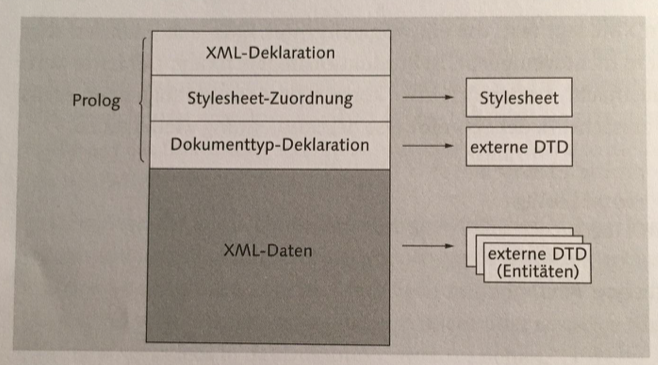
\includegraphics[scale=.5]{./images/Aufbauschema_eines_XML-Dockuments}
\captionof{figure}{Aufbauschema eines XML-Dockuments}

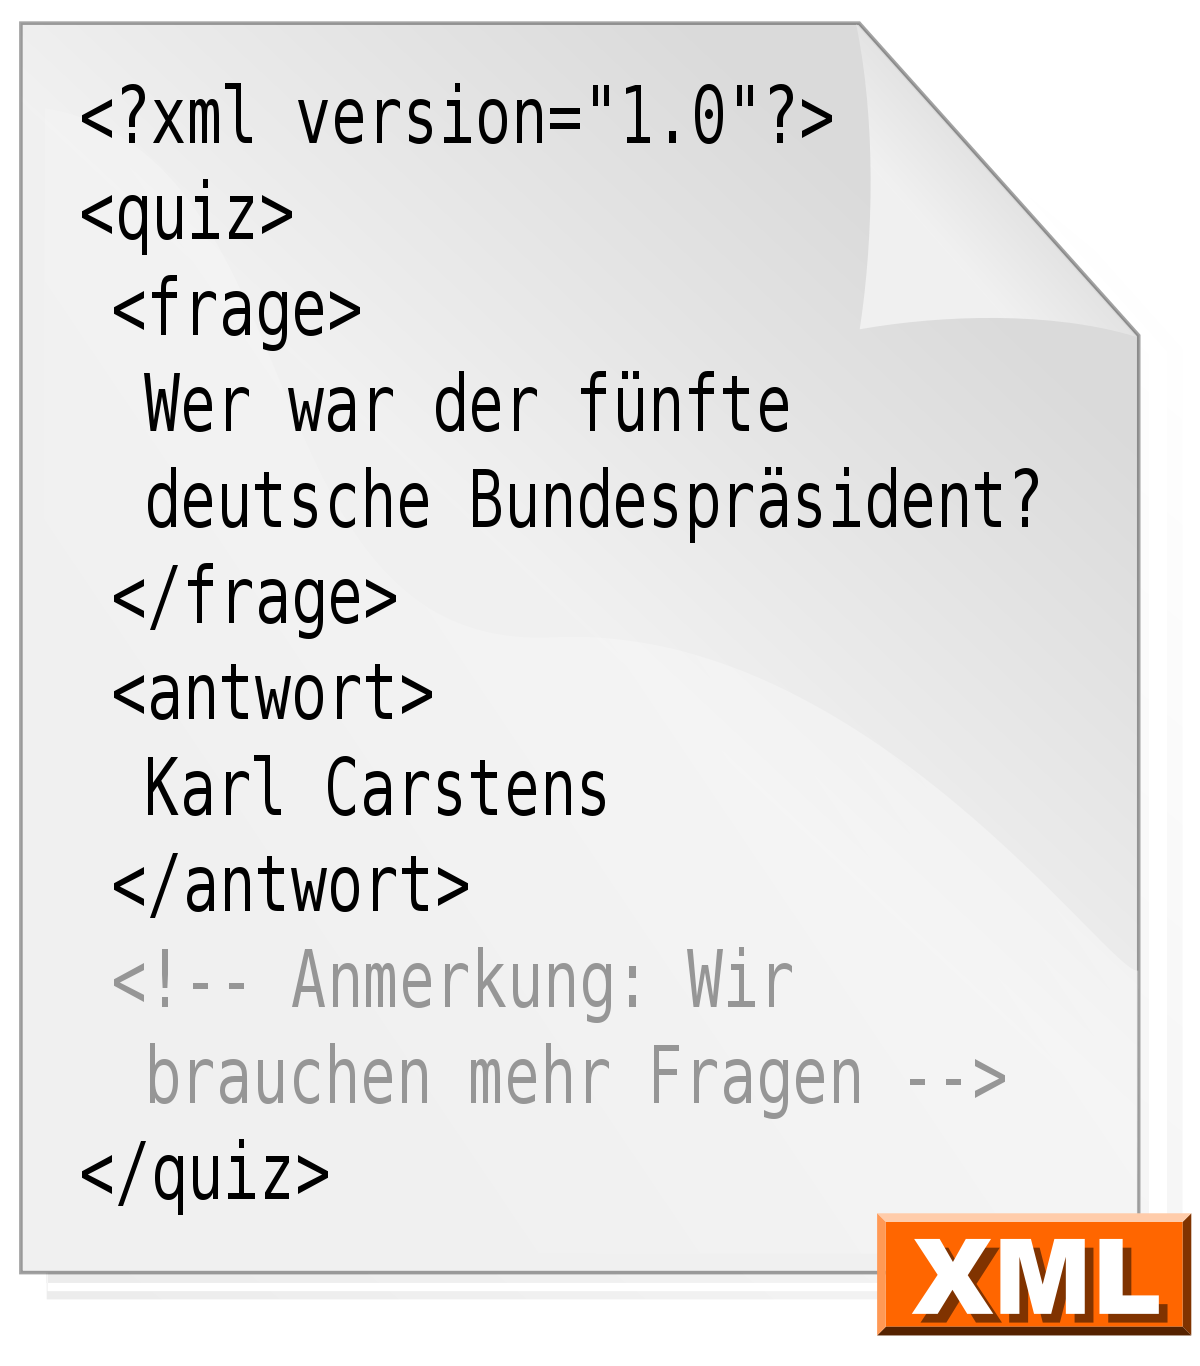
\includegraphics[scale=.3]{./images/Xml_datei_Beispiel}
\captionof{figure}{Beispiel einer XML-Datei}
\end{center}
\subsubsection{JSON}

JSON steht für JavaScript Object Notation und bezeichnet die kompakte Schreibweise von Objekt- und Arraystrukturen.\cite{philipp524} Es handelt sich um ein textuelles Daten Format, das von der Objekt Notation der JavaScript-sprache abgeleitet ist. es wird sehr gerne als Datentransportsprache zwischen Client und Server für Ajax-anfragen verwendet. Für einen schnellen Austausch wird es oft gegenüber XML bevorzugt. Werfen wir zuerst einen Blick auf die Geschichte von JSON. 

\textit{\textbf{Historik}}

Kurz nach Beginn des großen AJAX-Hypes im Jahr 2005 etablierte sich aus praktischen Gründen neben Klartext und XML quasi eine weiteres Übertragungsformat für die Kommunikation via AJAX: JSON, die JavaScript Objekt Notation.\cite{philipp658}
Der JSON wurde von Douglas Crockford zwischen 2002 und 2005 gebaut. Der erste JSON-Standard ist ECMA-404, der im Oktober 20032 veröffentlicht wurde. Derzeit wird er von zwei konkurrierenden Standards beschrieben: IETF RFC 82593 und ECMA-4044. Die neueste Version der Formatspezifikation stammt vom Dezember 2017. \cite{wikip01}

\textit{\textbf{Anwendung}}

Um ein vollständiges und konformes JSON zu erstellen, ist es notwendig, die richtige Syntax zu befolgen und das Dokument mit der Erweiterung .json zu speichern. Ein Json-Objekt beginnt und endet mit geschweiften Klammern {} und besteht im Wesentlichen aus zwei Teilen: Schlüssel und Werte. 

Die Schlüssel sind Zeichenketten, sie enthalten eine Folge von Zeichen, die von Anführungszeichen umgeben sind. Wert ist ein gültiger JSON-Datentyp. Es kann in Form eines Arrays, Objekts, einer Zeichenkette, eines booleschen Wertes, einer Zahl oder null vorliegen. Es kann zwei oder mehr Schlüssel/Wertpaare enthalten, die durch ein Komma getrennt sind. Auf jeden Schlüssel folgt ein Doppelpunkt, um ihn vom Wert zu unterscheiden. Mit diesem Bild ist es möglich, eine Darstellung eines Json zu beobachten. 

\begin{center}
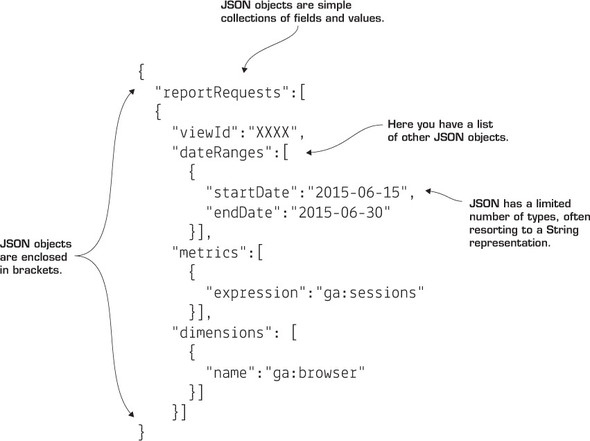
\includegraphics[scale=1]{images/Darstellung_eines_JSON-Objekts}
\captionof{figure}{Darstellung eines JSON-Objekts}
\end{center}

\subsubsection{BSON}

BSON ist eine Weiterentwicklung des Datenaustauschformates JSON der Firma 10gen und ist unter anderem ein fester Bestandteil von MongoDB. Die Libraries sind für viele Programmiersprachen bereits vorhanden. Da die BSON-Spezifikation öffentlich ist, kann BSON auch für andere Projekte genutzt werden.\cite{thKloeln}

BSON ist so konzipiert, dass es im Raum effektiv ist, aber in einigen Fällen ist es nicht viel effektiver als JSON. In einigen Fällen benötigt BSON sogar mehr Platz als JSON. Der Grund dafür ist ein weiteres Designziel von BSON: die Kreuzbarkeit. BSON fügt den Dokumenten zusätzliche Informationen hinzu, wie z. B. die Länge von Strings und Unterobjekten. Dadurch wird die Traversierung schneller.\cite{bson} BSON ist außerdem so konzipiert, dass es sich schnell kodieren und dekodieren lässt. Ganzzahlen werden z. B. als 32- (oder 64-) Bit-Ganzzahlen gespeichert, so dass sie nicht in und aus dem Text geparst werden müssen. Dies verbraucht mehr Speicherplatz als JSON für kleine ganze Zahlen, aber es ist viel schneller zu parsen. Neben der Kompaktheit fügt BSON zusätzliche Datentypen hinzu, die in JSON nicht verfügbar sind, darunter die Datentypen BinData und Date.“
\subsection{Programmierparadigmen für Webanwendungen}
\subsubsection{SOAP}
SOAP steht für Simple Object Access Protocoll und wurde von DevelopMentor, IBM, Lotus Development Corp, Microsoft, Userland Software entwickelt. Der Hauptautor ist Don Box von DevelopMentor, einer der Autoren des XML-Manifests. SOAP ist ein Standard, der vom W3C-Konsortium unterstützt wird. In der Welt der Web-Service-Technologie steht SOAP für ein standardisiertes Paketprotokoll zum Nachrichtenaustausch zwischen verteilten Systemen. Diese Spezifikation definiert eine einfache xml-basierte Umgebung (envelope) zum Austausch von Informationen und einen Satz von Regeln zur Übersetzung von Anwendungen und plattformspezifischen Datentypen in XML-Darstellungen. SOAP ist so konzipiert, dass es eine Vielzahl von Anwendungsfällen unterstützt.\cite{saop1}

\textit{\textbf{Historik}}

Einer der Hauptakteure bei der Emanzipation von Web-Services-Technologien auf der Java-Plattform ist IBM. IBM hat außerdem eine der allerersten Implementierungen der SOAP-Spezifikation für Java auf den Markt gebracht, die in der Java-Entwicklergemeinde auf großes Interesse gestoßen ist. Seitdem konzentriert sich IBM auf die Fähigkeiten dieser Gemeinschaft, um den Erfolg und die Nachhaltigkeit des Frameworks sicherzustellen. Daher beschloss IBM in der zweiten Hälfte des Jahres 2000, SOAP der Open-Source-Welt zu schenken, insbesondere der Apache Fundation.

Das Apache SOAP-Framework von IBM, das in Apache umbenannt wurde, hat eine Reihe von Weiterentwicklungen und Verbesserungen erfahren und war ein großer Erfolg. Infolgedessen hat Sun Apache SOAP schnell als Apache SOAP Framework in seine J2EE-Applikationsserver integriert. Apache SOAP Version 2.2 wurde im Mai 2001 veröffentlicht und danach gab es keine weitere Entwicklung dieses Frameworks. Nachdem das SOAP Framework das Ende seiner Lebensdauer erreicht zu haben scheint, werden sich im kommenden Jahr alle Anstrengungen auf den Nachfolger von Apache SOAP konzentrieren.

\textit{\textbf{Anwendung}}

Die schon im Namen explizit betonte Einfachheit des Protokolls ist dabei ausdrückliches Designziel. Es geht darum, einen unkomplizierten Rahmen für die Nachrichten Übermittlung zwischen Anwendungen bereitzustellen, ohne zu enge Festlegungen über die Art des Nachrichtentransports oder die Anwendungen selbst zu treffen, die das Protokoll nutzen wollen. Dazu wurde eine kleines XML-Vokabular entwickelt, das hauptsächlich angibt, wie die Nachrichten verpackt werden. Ein SOAP-Nachricht ist zunächst ein ganz normales XML-Dokument, das mit den üblichen XML-Prozessoren verarbeitet werden kann. Der Spezifikationsentwurf schreibt als äußeren Rahmen eine <envelope>-Element vor, also einen Umschlag, in den alles andere hineingepackt wird. Optional ist ein SOAP-Header, vorgeschrieben dagegen ein SOAP-Body, der den eigentlichen Inhalt der Nachricht enthält.\cite{helmut529_30}

\begin{center}
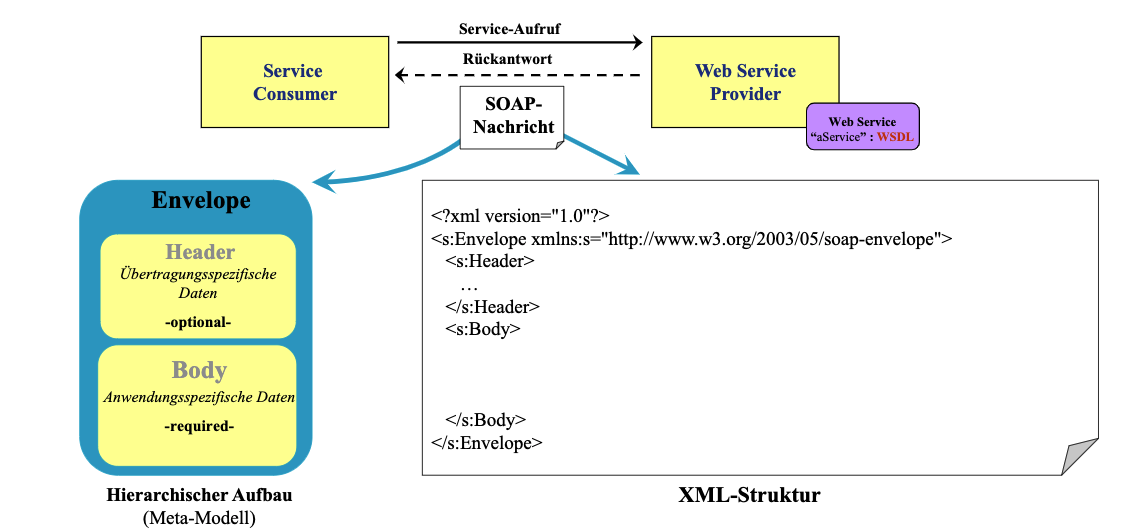
\includegraphics[scale=.4]{images/Struktur_ein_SOAP}
\captionof{figure}{Struktur ein SOAP}
\end{center}

\subsubsection{REST API}
Damit wir die RestFull Api verstehen, fangen wir erst wieder mit den Definitionen ein.
Ein REST stellt einen alternativen Ansatz für die Realisierung von Web Services dar.“ Eine Rest API ist eine Schnittstelle, über die Sie die Kommunikation zwischen Ihrem Computer und einem Server herstellen können, damit dieser Ihnen Daten zur Verfügung stellt. Rest-API ist die an der häufigsten verwendeten Art von API im Webbereich. REST steht für Representational State Transfert.\cite{alda}

\textit{\textbf{Historik}}

Vor den 2000er Jahren gab es keine Standards dafür, wie man eine API entwirft oder gar verwendet. Die Integration von APIs erforderte die Verwendung von Protokollen, wie z. B. SOAP, die notorisch komplex in der Erstellung, Verwaltung und Fehlersuche sind. Das alles änderte sich in den 2000er Jahren, als das wahre Potenzial von Web-APIs erkannt wurde. Eine Gruppe von Experten, angeführt von Roy Fielding, erfand REST und veränderte die API-Landschaft für immer.
Das Ziel war es, einen einfachen Standard zu schaffen, der es zwei Servern ermöglicht, miteinander zu kommunizieren und Daten auszutauschen, egal wo auf der Welt sie sich befinden. Sie schufen eine Reihe von Prinzipien, Eigenschaften und Einschränkungen, die REST genannt werden, sowie eine ressourcen-orientierte Architektur: einheitliche Schnittstelle, Client/Server-Architektur, keines Zustands, Implementierung der Ressourcen-darstellung, Verwendung von HTTP und HTTP-Methoden.

\textit{\textbf{Anwendung}}

Eine API wird oft mit dem Server oder der Datenbank verwechselt, aber in Wirklichkeit handelt es sich um den Code, der den Server anweist, bestimmte Aktionen entsprechend der gestellten Anfrage auszuführen. Es handelt sich also einfach um ein Interface (Application Programming Interface).
Der Zugriff auf den Rest der API erfolgt über HTTP-Methoden (GET, POST DELETE, PUT). Dadurch ist es möglich, einen Server mit einer vom Ersteller der API bereitgestellten URL durch eine einfache HTTP-Anfrage zu interagieren. Eine HTTP-Anfrage an einen Server provoziert jedoch eine Antwort, je nach Erfolg (Code: 200) oder Misserfolg der Operation (403, 404, 500, 504 ...). Es ist möglich, die Daten Allgemeinen im JSON-Format zu erhalten.

\begin{center}
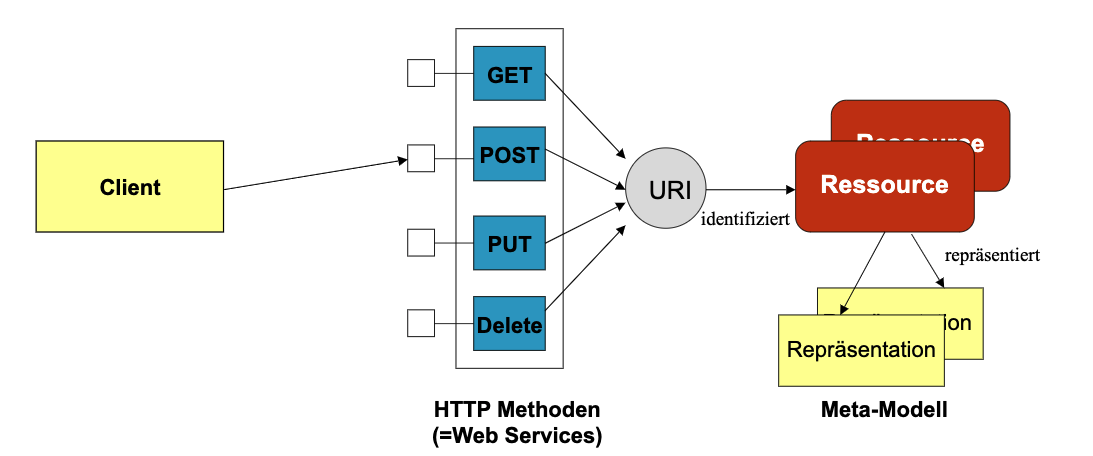
\includegraphics[scale=.3]{images/Aufbau_eine REST-basierten_Web_Services_Architektur}
\captionof{figure}{Aufbau eine REST-basierten Web Services Architektur}
\end{center}

\subsubsection{GraphQL}

GraphQL ist eine Abfragesprache für APIs und eine Laufzeitumgebung zur Erfüllung dieser Abfragen mit Ihren vorhandenen Daten. GraphQL bietet eine vollständige und verständliche Beschreibung der Daten in Ihrer API, gibt Kunden die Möglichkeit, genau das anzufordern, was sie benötigen, und nicht mehr, erleichtert die Weiterentwicklung von APIs im Laufe der Zeit und ermöglicht leistungsstarke Entwicklerwerkzeuge.\cite{graphQL}

\textit{\textbf{Historik}}

Bis 2012 wird die Verbreitung von Mobiltelefonen weltweit monströse Zahlen erreichen. Es ist eine solche Invasion, dass Unternehmen, die ihre Produkte nicht anpassen, gefährdet sind. An diesem Punkt ist Facebook gefährdet. Facebook geht online. Als Ergebnis haben sie ihre IOS-App wie eine Website gemacht, in Web-Ansicht. Sehr schnell merken sie, dass es (zu diesem Zeitpunkt) ein bisschen scheiße ist. Also entschied man sich, es komplett in nativer Sprache neu zu erstellen, um ein besseres Kundenerlebnis zu schaffen. Sofort wurde ihnen eine weitere Wand vor die Nase gesetzt. Die bestehende Architektur funktioniert nicht. Hauptsächlich, weil die Endpunkte ihrer bestehenden REST-API keine Flexibilität bei den Daten zulassen. Für verschachtelte Daten sind mehrere Roundtrips zu verschiedenen Endpunkten erforderlich, was zu Langsamkeit und Inkonsistenzen führt. Ein Teil der Nutzdaten wird für die meisten Abfragen nicht benötigt, was zu unnötigen Datenübertragungen führt. Und vor allem ist es für Facebook mühsam, so viele HTTP-Aufrufe zu verarbeiten.
In diesem infernalischen Kontext reservieren Lee Byron, Dan Schafer und Nick Schrock im Februar 2012 Büros in einer Ecke von Facebook. Sehr schnell wird ein erster Prototyp von GraphQL, damals SuperGraph genannt, von unseren drei Entwicklern erstellt. Im August 2012 wird GraphQL in der Produktion mit der neuen nativen Facebook-App ausgeliefert. Im Jahr 2015 erscheint die erste öffentliche Version im Internet. GraphQL ist auch heute noch präsent, wenn Sie auf Ihrer Facebook-Pinnwand scrollen.\cite{graphQL2}

\textit{\textbf{Anwendung}}

Mit GraphQL kann man Daten auf einfache, flexible und sehr präzise Weise manipulieren. GraphQL ist keine Programmiersprache und kein Framework, sondern eine Spezifikation zur Implementierung einer API.
GrapQL macht das Leben einfacher, denn damit müssen Sie nur eine Post request Anfrage stellen, die nach genau dem fragt, was man genau braucht, als Antwort gibt es die Ressourcen zurück, die nach dem Aufbau Ihres GraphQL Anfrage. Der kleine Unterschied zu REST ist, dass man bei REST von den Endpunkten definierte Objekte bekommt, bei GraphQL hingegen passt man sich nicht an ein vom Backend bereits vordefiniertes Objekt an, sondern man definiert dynamisch, was man auf der Frontend Seite erhalten möchte. 
Das folgende Bild von der Startseite der offiziellen GrapQL-Website stellt die Funktion von GraphQL übersichtlich und einfach dar.

\begin{center}
\includegraphics[scale=.4]{images/Globaler_ueberblick über_GraphQL}
\captionof{figure}{Globaler Überblick über GraphQL}
\end{center}


